\chapter{Einführung Machine Learning}
\label{chap:einführungMachineLearning}
Um sich mit Machine Learning auseinanderzusetzen, muss zunächst die Theorie verstanden werden, welche sich dahinter verbirgt. Anders als bei herkömmlicher Programmierung, in der ein Programm und Daten einen Output erzeugt, leitet man beim Machine Learning aus gesammelten Daten und Outputs ein Programm her \cite[S.~3]{WML}.  Dies wird in der unten stehenden Grafik verdeutlicht.
\newline

\begin{figure}
	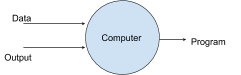
\includegraphics[]{C:/Users/PitAu/Desktop/Seminar Zeug/MLSKLSeminar/LaTex/Bilder/sBdyby6FyPckxbimKufRD4Q.png}
	\caption{Machine Learning}\cite[S.~3]{WML}
\end{figure}
\begin{figure}
	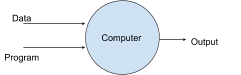
\includegraphics[]{C:/Users/PitAu/Desktop/Seminar Zeug/MLSKLSeminar/LaTex/Bilder/sZFI1L7gymY3C_ipjtqSvrg.png}
	\caption{Herkömmliche Programmierung}\cite[S.~3]{WML}
\end{figure}


\chapter{Einführung verschiedener Problemstellungen}
\label{chap:einführungProblemstellungen}
Nicht nur bei den Algorithmen gibt es verschiedene Unterteilungen, auch die Probleme, welche man mit Machine Learning lösen möchte, lassen sich in 3 Hauptkategorien unterteilen.

\section{Classification}
\label{sec:classification}
In diesen Fällen versucht man mit hilfe von Machine Learning zu ermitteln in was für eine Kategorie ein Objekt gehört\cite{SKL}. Dies realisiert man, indem man das System mit einem Dataset der möglichen Kategorien trainiert. Das Ergebnis eines Classification Problems ist entweder ein diskreter oder ein kontinuierlicher Wert \cite[S.~4]{WML}. Spamfilter wären ein Beispiel eines Classification Problem, in dem Mails beispielsweise in die Kategorien Spam und kein Spam eingeteilt werden könnten. 

\subsection{Support Vector Machine (SVM)}
\label{sec:SVM}
Ziel des SVM Algorithmus ist es, eine Hyperebene(Ebene mit n-1 Dimensionen) in einen n-dimensionalen Raum zu legen (wobei n die Anzahl der Features ist), sodass alle Datensätze einer Klasse auf einer Seiter der Hyperebene liegen und alle Datensätze einer anderen Klasse auf der anderen Seite. Dann kann für neue Daten aufgrund ihrer Position in Beziehung zu Ebene bestimmt werden, welcher Klasse diese angehört \cite[S.~177f.]{WML}.

\subsection{Random Forest Classifier}
\label{sec:RFC}
<<<<<<< HEAD
Bei diesem Algorithmus  werden aus dem Trainingsset zufällig Teilmengen genommen,mit denen verschiedene Modelle trainiert werden\cite[S.~256]{MB}. Diese verschiedenen Modelle werden durch Decisiontrees trainiert. Später kommt es durch ein “Mehrheitsvotum” zu einer finalen Einordnung der Klasse\cite{MED}.  Dies wird in folgender Abbildung verdeutlicht.

\begin{figure}
	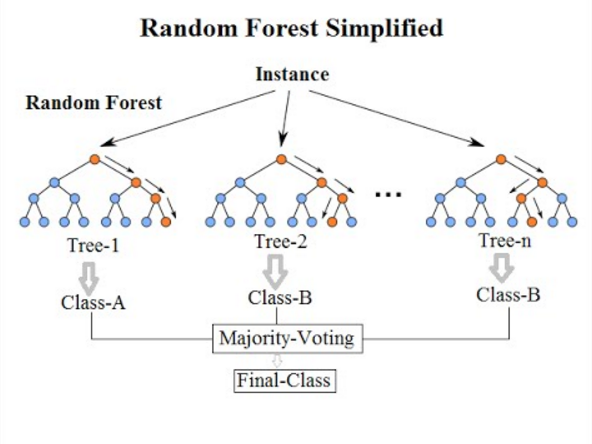
\includegraphics[width=1.0\textwidth]{C:/Users/PitAu/Desktop/Seminar Zeug/MLSKLSeminar/LaTex/Bilder/1_i0o8mjFfCn-uD79-F1Cqkw.png}
	\caption{Diagramm: Random Forrest}
\end{figure}
=======
Bei diesem Algorithmus  werden aus dem Trainingsset zufällige Teilmengen genommen,mit denen dann mehrere Decisiontrees trainiert werden. Daher auch der Name "Random Forest", da dieser aus vielen verschiedenen Bäumen besteht\cite[p.~256]{MB}. Bekommt dieser Algorithmus einen Input gibt er ihn an jeden einzelnen Tree weiter, jeder für sich fällt dann unabhängig seine eigene Entscheidung. Später kommt es durch ein “Mehrheitsvotum” der einzelnen Trees zu einer finalen Einordnung der Klasse, wodurch dieser Algorithmus deutlich weniger anfällig für Overfitting ist als ein einzelner Decisiontree\cite{MED}. \hyperlink{einführungMachineLearning}{[Grafik Random Forest]}
>>>>>>> 1256aa2475e4a5bcfd169577550135e3e87f4ce8

\section{Regression}
\label{sec:regression}
Hier wird versucht mit Machine Learning eine Prognose zu machen. Diese Prognose entsteht, indem die KI verschiedene Variablen in Beziehung setzt und dadurch eine Vorhersage ermittelt. Als Ergebnis liefert die KI in diesem Fall einen kontinuierlichen Output \cite[S.~4.]{WML}.  Ein typisches Beispiel für Regression ist beispielsweise die Vorhersage der erreichten Punktzahl in einem Test im Verhältnis zur Lerndauer in Stunden.  Dies wird in folgender Abbildung verdeutlicht.
\begin{figure}
	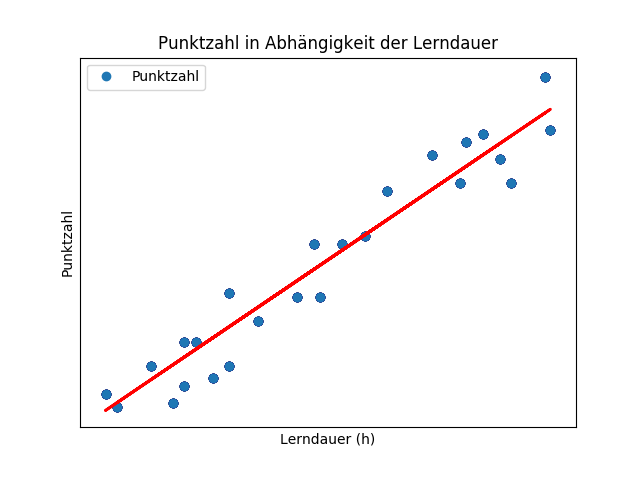
\includegraphics[width=1.0\textwidth]{C:/Users/PitAu/Desktop/Seminar Zeug/MLSKLSeminar/LaTex/Bilder/machine_learning_regression_with_line.png}
	\caption{Diagramm: Regression}
\end{figure}

\subsection{Lineare Regression}
\label{sec:lineareRegression}
Gilt als ein sehr einfacher Algorithmus, bei dem versucht wird eine lineare Annäherung zwischen einer Abhängigen und einer Unabhängigen Variablen zu ermitteln\cite[S.~100.]{WML}.  


\subsection{Decisiontree Regression}
\label{sec:decisiontreeRegression}
Decisiontrees werden bei classification und regression Problemen eingesetzt. Ziel dieses Algorithmus ist es, von einem Dataset Regeln zu lernen und anhand dieser Vorhersagen zu machen.Der Decisontree wird genauer, wenn dieser größer wird oder die Auswahlmöglichkeiten (decisions) komplexer werden\cite{SKLT}.

\subsection{Random Forest Regression}
\label{sec:randomForestRegression}
Dieser Algorithmus funktioniert wie der vorher schon genannte Random Forest Classifier, nur mit dem unterschied, dass am ende keine Finale Klasse entsteht, sonder ein kontinuirlicher Output. Um diesen zu erreichen wird anders als beim Random Forest Classifier bei der Abstimmung kein Majority-Voting durchgeführt, sondern es wird der Mittelwert der Ergebnisse von den verschiedenen Decision Trees gebildet.

\section{Clustering}
\label{sec:clustering}
Bei Clustering Problemen wird versucht mit hilfe von Machine Learning verschiedene Daten aus einem Dataset in verschiedene Gruppierungen einzuordnen\cite[S.~5.]{WML}. Clustering Probleme treten dann auf, wenn z.B. jemand eine Kundenanalyse durchführen möchte. Solch eine Kundenanalyse kann aufschlussreich sein, um das Kaufverhalten verschiedener Arten von Kunden zu analysieren.


\subsection{K-Means}
\label{sec:kMeans}
K-Means wird bei einem unlabeled Dataset angewendet und versucht in diesem K Gruppen zu finden. Dazu werden zunächst k zufällige Datenpunkte ausgewählt und dann anhand dieser die restlichen Daten zu den Clustern zugeordnet. Anschließend wird der Mittelwert(Mean) jedes Clusters bestimmt und die Daten werden anhand der neuen Means zu Clustern zugeordnet. Dieser Vorgang wird wiederholt, bis sich die Mittelwerte nicht mehr ändern. Bei K-Means werden beliebig viele solcher Modelle erstellt, und am Ende das verwendet, welches die geringste Varianz bietet\cite[S.~222.]{WML}.


\section{Overfitting/Underfitting}
\label{sec:overfittingUnderfitting}
Damit man durch die genannten Algorithmen ein vernünftiges Ergebnis erzielen kann muss man beachten, dass die KI nicht overfittet oder underfittet, da es so zu unbrauchbaren Ergebnissen kommt.


\subsection{Overfitting}
\label{sec:overfitting}
Beim Overfitting wurde das Modell so trainiert, dass es versucht jeden einzelnen Punkt aus den Trainingsdaten zu berücksichtigen. So werden auch unwichtige schwankungen der Daten beachtet. Bei Modellen die overfitten ist das größte Problem, dass dieses Modell nicht für neue Daten geeignet ist\cite[S.~214.]{WML}.


\subsection{Underfitting}
\label{sec:underfitting}
Anders als beim Overfitting passiert bei Underfitting im Prinzip das Gegenteil und das Modell schafft es nicht den Verlauf der Daten zu erfassen\cite[S.~214.]{WML}.
Ziel ist es ein Modell zu finden, welches sich zwischen Overfitting und Underfitting befindet. Die unten abgebildeten Graphen sind jeweils ein Beispiel für Underfitting, Overfitting und einem Modell, welches erstrebenswert ist. Das Modell Degree 1 ist das Modell, welches underfittet, das Modell Degree 4 ist das angestrebte und das Degree 15 das overfittete Modell.
\newline
\begin{figure}
	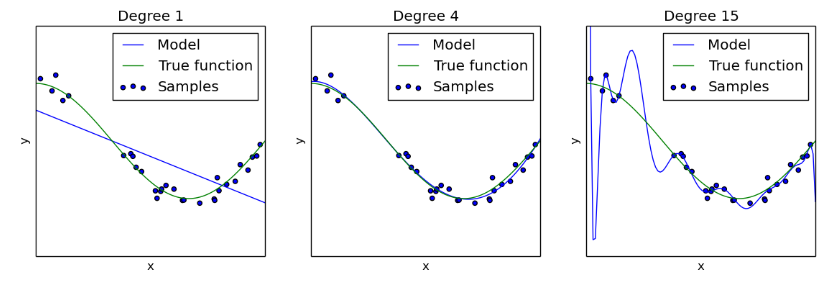
\includegraphics[width=1.0\textwidth]{C:/Users/PitAu/Desktop/Seminar Zeug/MLSKLSeminar/LaTex/Bilder/OverUnderfitting.PNG}
	\caption{Overfitting Underfitting}
\end{figure}


\section{Performance Measure}
\label{sec:performanceMeasure}
Um die Genauigkeit der verschiedenen Algorithmen vergleichen zu können, muss eine Formel zur Bestimmung der Fehler gewählt werden. 
Die übliche Methode ist der “Root Mean Spuare Error”. Diese gibt einen Ausblick auf die Anzahl an Fehler, die das System typischerweise macht, wobei größere Fehler auch schwerer gewichtet werden\cite[S.~39.]{AG}.
\newline
\begin{figure}
	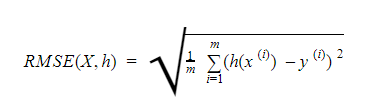
\includegraphics[]{C:/Users/PitAu/Desktop/Seminar Zeug/MLSKLSeminar/LaTex/Bilder/Berechnung.PNG}
	\caption{Berechnung des Root Mean Square Error}
\end{figure}


\chapter{SciKit-Learn}
\label{chap:sciKitLearn}
Scikit-Learn ist ein Projekt, welches 2007 von David Cournapeau gestartet wurde\cite{SKL}. Ziel dieses Projektes ist es Machine-Learning für jeden zu vereinfachen, indem sie verschiedene Python-Libraries erstellen. Da die Algorithmen des Machine-Learning nur durch sehr komplex Berechnungen zu realisieren sind, stellt scikit verschiedene Libraries zur verfügung, welche diese komplexen Berechnungen für den Programmierer übernimmt, so dass oftmals nur wenige Funktionsaufrufe nötig sind, um eine KI zu erstellen. Aber scikit besteht nicht nur aus Funktionen, welche komplexe Berechnungen durchführen, es gibt auch Funktionen, wie z.B. train\_est\_split(), welche festlegt, welche Daten zum trainieren und welche zum Testen genommen werden.

\chapter{Beispielprojekt}
\label{chap:Beispielprojekt}

\section{Projektvorstellung}
\label{sec:projektvorstellung}
Um die beschriebenen Herangehensweisen aus dem vorherigen Kapitel besser verstehen und nachvollziehen zu können, soll in diesem Kapitel ein eigenes Projekt durchgeführt werden. Dieses wird uns sowohl mit der Umsetzung der oben beschriebenen Konzepte bekannt machen, also auch eine grundlegende Einführung in die Funktion von SciKit-Learn ermöglichen. 
Um einen Überblick über dieses umfassende Thema zu bekommen, werden zunächst die drei verschiedenen Herangehensweisen(Classification, Regression und Clustering) jeweils mit zwei verschiedenen Algorithmen implementiert. So werden die Unterschiede und Gemeinsamkeiten herausgearbeitet, um ein Vergleich der einzelnen Implementierungen zu ermöglichen. Hierbei muss natürlich bedacht werden, dass sich für jedes Dataset andere Algorithmen und Herangehensweisen als am besten geeignet erweisen: Um die Werte einer linearen Funktion zu bestimmen eignet sich vermutlich eher eine Regression als eine Classification oder Clustering. Doch genau diese Fragestellungen sollen in diesem Projekt behandelt und beantwortet werden.
Zunächst wird dazu ein Experiment aus “Hands-On Machine Learning with SciKit-Learn” nachgestellt, und dann mit eigenen Ansätzen weitergearbeitet.

\section{Datensatz}
\label{sec:datensatz}
Für das Projekt wurde der “California Housing Prices” Datensatz gewählt. Dieser stammt aus R. Kelly Pace’s and Ronalds Berry’s “Sparse Spatial Autoregressions” Statistics \& Probability Letters 33 no. 3 (1997). Wie der Name schon vermuten lässt handelt es sich bei diesen Daten um die Preise für eine Haus in Kalifornien in Abhängigkeit von dessen Lage. Die Werte stammen aus 1990  und sind somit nicht mehr relevant, dennoch bieten sich viele Möglichkeiten an diesen Daten zu lernen und zu experimentieren, für das geplante Projekt also die perfekten Voraussetzungen.

\section{Vorbereiten der Entwicklungsumgebung}
\label{sec:vorbereitenEntwicklungsumgebung}
Auf dem für das Projekt zur Verfügung stehenden Computer muss Python mit folgenden Modulen installiert sein: 
\begin{itemize}
\item jupyter
\item matplotlib
\item numpy
\item pandas
\item scipy
\item scikit-learn
\end{itemize}
Zusätzlich wird das Modul virtualenv installiert um das Projekt in einer isolierten Umgebung durchführen zu können. Als letztes wird der Jupyter-Server gestartet.

\chapter{Projektdurchführung}
\label{chap:projektdurchführung}
Das Jupyter-Notebook das zur Durchführung dieses Projekts angelegt wurde kann unter \href{https://github.com/robbmue/MLSKLSeminar}{https://github.com/robbmue/MLSKLSeminar} eingesehen werden.
In diesem Kapitel werden als erstes die Daten aus dem Datensatz importiert und aufgearbeitet. Dann werden die Daten visualisiert und mithilfe der aus der Visualisieren gewonnenen Kentnisse in eine sogenannte Pipeline überführt, welche die Aufbereitung der Daten übernimmt.
Anschließend können dann unterschiedliche Algorithmen aus den Feldern Regression und Classification mit Diesen trainiert und verglichen werden, eine Überprüfung der Ergebnisse mithilfe von Cross-Validation und eine abschließende Evaluation durchgeführt werden.

\section{Vorbereitung der Daten 1}
\label{VorbereitungDerDaten1}
Zunächst muss der Datensatz, der verwendet werden soll in das System importiert werden, wofür der vorbereiteten Datensatz aus “Hands on Machine Learning” verwenden konnte\cite{DATA}. Die Daten müssen anschließend entpackt werden und können dann mithilfe von pandas eingelesen werden. 
Anschließend können Informationen über den Datensatz angezeigt werden. Diese finden sich im der Abbildung Attribut Datensatz. Dort lässt sich erkennen, dass der Datensatz 20640 Einträge enthält. Eine Ausnahme bildet dabei das Attribut “total\_bedrooms”. Diese Problem wird in Kapitel 6.3 Vorbereitung der Daten 2 behandelt.
Um eine genauere Vorstellung des Datensatzes zu bekommen, mit dem gearbeitet wird, kann außerdem ein Histogramm erstellt werden. Dieses findet sich in der Abbildung Histogramm. 
Dann muss dann das zur Verfügung stehende Dataset in zwei aufgesplittet werden. Ein Richtwert für die Aufteilung ist 80/20: 80\% der Daten befinden sich nach dem Split im train\_set und 20\% im test\_set.
Zuletzt soll das Income-Feature in Kategorien eingeteilt werden, da dieses Feature für das Endergebnis eine besonders große Rolle spielt. Hier wurde eine Aufteilung in 5 Schichten gewählt, wobei jede ein Einkommen von +\$15,000 repräsentiert. 
Also \$0 - \$15,000, \$15,000 - \$30,000 usw. wobei die letzte Kategorie nach oben nicht begrenzt ist, also >\$60,000. Ein Histogramm dieser Kategorien ist das Histogramm Verteilung Income. Mithilfe dieser Kategorien und des StratisfiedShuffleSplits, den scikit-learn zur Verfügung stellt, können Train und Test Sets gebildet werden, die die Verteilung der Einkommensschichten repräsentieren können. Diese werden strat\_train\_set und strat\_test\_set genannt.

\begin{figure}
	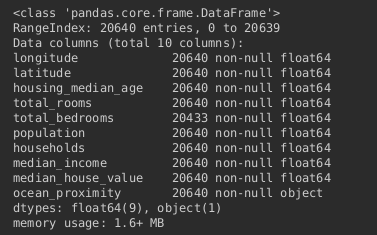
\includegraphics[]{C:/Users/PitAu/Desktop/Seminar Zeug/MLSKLSeminar/LaTex/Bilder/pasted image 0 (8).png}
	\caption{Attribute Datensatz}
\end{figure}
\begin{figure}
	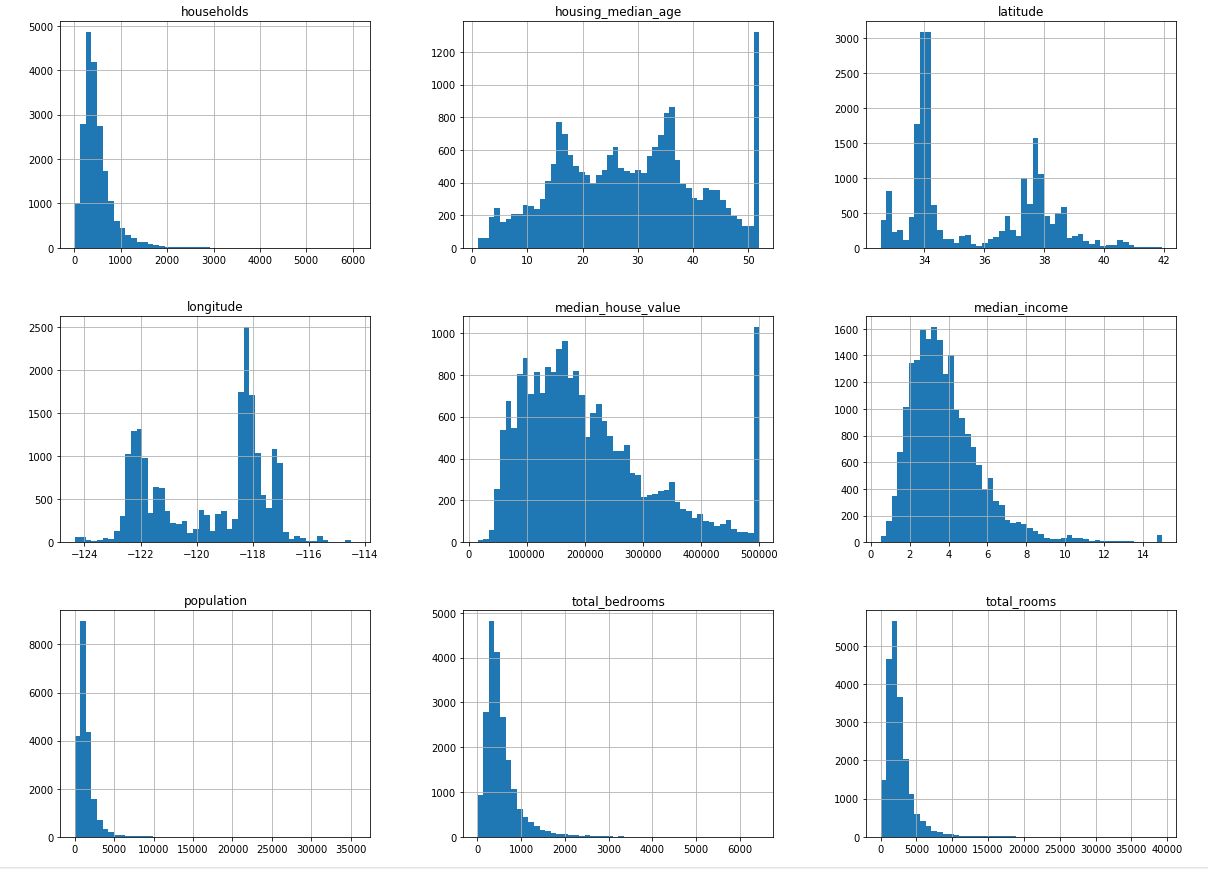
\includegraphics[width=1.0\textwidth]{C:/Users/PitAu/Desktop/Seminar Zeug/MLSKLSeminar/LaTex/Bilder/pasted image 0 (9).png}
	\caption{Histogramm}
\end{figure}
\begin{figure}
	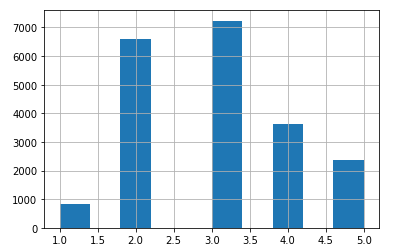
\includegraphics[width=1.0\textwidth]{C:/Users/PitAu/Desktop/Seminar Zeug/MLSKLSeminar/LaTex/Bilder/pasted image 0 (10).png}
	\caption{Histogramm: Verteilung Income}
\end{figure}


\section{Visualisierung der Daten}
\label{visualisierungDerDaten}
Um ein noch besseres Verständnis für die Daten zu bekommen werden diese auf verschiedene Arten visualisiert. Als Erstes als die reine Verteilung unserer Daten auf den Raum Kalifornien. Jedes Datum wird mit einem Punkte repräsentiert, dicht besiedelte Gebiete werden hervorgehoben. Da als X- und Y-Achsen die Koordinaten gewählt wurden, wird hier die Form Kaliforniens abgebildet. Dies ist in der Grafik Räumliche Verteilung der Datensätze wiederzufinden.
\begin{figure}
	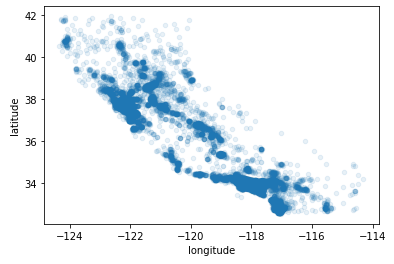
\includegraphics[width=1.0\textwidth]{C:/Users/PitAu/Desktop/Seminar Zeug/MLSKLSeminar/LaTex/Bilder/pasted image 0 (11).png}
	\caption{Räumliche Verteilung der Datensätze}
\end{figure}

Damit die Muster, die dieser Grafik zugrunde liegen noch besser verstanden werden können, werden sie in eine Jet-Grafik umgewandelt. Rot symbolisiert dabei die hohen Grundstückspreise und Blau die niedrigen.

\begin{figure}
	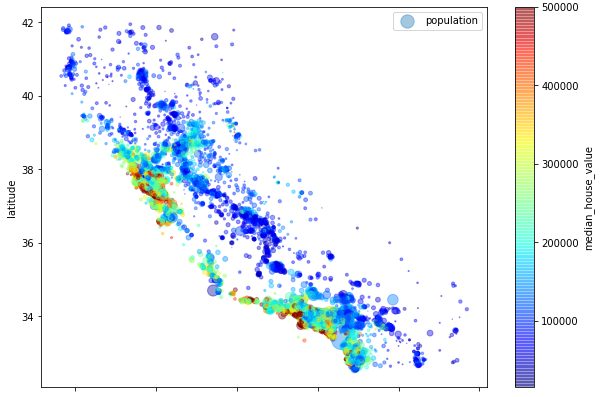
\includegraphics[width=1.0\textwidth]{C:/Users/PitAu/Desktop/Seminar Zeug/MLSKLSeminar/LaTex/Bilder/pasted image 0.png}
	\caption{Hier lässt sich erkennen, dass für unser vorhaben vor allem die Attribute Lage und Bevölkerungsdichte wichtig sein werden. Mithilfe dieser Visualisierungen lassen sich also wichtige Informationen herausarbeiten.
}
\end{figure}


\section{Vorbereitung der Daten 2}
\label{VorbereitungDerDaten2}
Mithilfe dieser Informationen können die Daten weiterverarbeitet werden. 
Dafür konnten die von scikit-learn implementierten Module Pipeline, StandardScaler, ColumnTransformer und OneHotEncoder genutzt werden, auf deren Funktion hier nicht weiter eingegangen werden soll, das der Schwerpunkt des Projekts auf dem Vergleich der Machine-Learning-Algorithmen liegen soll und nicht auf dem Vorbereiten der Daten. Deswegen an dieser Stelle nur ein kurzer Überblick über die durchgeführten Schritte:
\begin{enumerate}
\item Die nicht vorhandenen total\_bedrooms Werte werden mit dem Mittelwerte aller total\_bedrooms befüllt
\item Es werden aus den vorhandenen Attributen neue, sinnvollere Attribute gebildet. Zum Beispiel ist das Attribut rooms\_per\_household deutlich sinnvoller als die einzelnen Attribute total\_roooms oder total\_households pro District.
\item Alle Werte werden standardisiert, was bedeutet dass der Mittelwert eines Attributes immer 0 ist, und die restliches Werte entsprechend um diesen gebildet werden.
\item Auf den nicht numerischen Wert ocean\_proximity wird der OneHotEncoder angewandt: Es wird ein Binärer Wert erzeugt, der den verschiedenen Kategorien entsprechend viele Stellen erhält. Für jede Kategorie wird dann also einer dieser Werte zu 1.
\end{enumerate}

\section{Durchfühurng Linear Regression}
\label{durchfühurngLinearRegression}
Folgendes Code Beispiel soll veranschaulichen wie simpel es mithilfe von scikit-learn ist, einen Machine-Learning Algorithmus zu trainieren:
\begin{figure}
	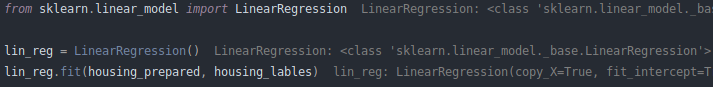
\includegraphics[width=1.0\textwidth]{C:/Users/PitAu/Desktop/Seminar Zeug/MLSKLSeminar/LaTex/Bilder/pasted image 0 (1).png}
	\caption{Code: Lineare Regression}
\end{figure}
Mit diesen wenigen Zeilen wurde zunächst das entsprechende Modul importiert, dann ein entsprechendes Objekt erzeugt und trainiert. 
Auch die Evaluierung des Systems ist nicht viel komplexer:
\newline
\begin{figure}
	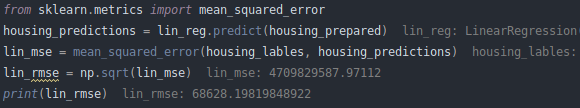
\includegraphics[width=1.0\textwidth]{C:/Users/PitAu/Desktop/Seminar Zeug/MLSKLSeminar/LaTex/Bilder/pasted image 0 (2).png}
	\caption{Code: Evaluation Regression}
\end{figure}

\section{Durchführung Decision Tree Regression \& Random Forest Regression}
\label{durchführungDecisionTreeRegressionRandomForestRegression}
Auch für diese Alternative bietet scikit-learn eine Implementation:
\newline
\begin{figure}
	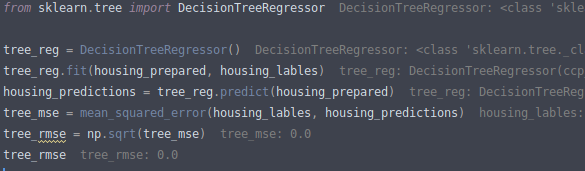
\includegraphics[width=1.0\textwidth]{C:/Users/PitAu/Desktop/Seminar Zeug/MLSKLSeminar/LaTex/Bilder/pasted image 0 (3).png}
	\caption{Code: Decision Tree Regression}
\end{figure}
Random Forest ist genauso zu implementieren, deswegen hier nicht abgebildet.

\section{Cross-Validation}
\label{crossValidation}
Beim validieren des Decision-Trees fällt natürlich auf, dass nach dem Abgleich der Ergebnisse ein RMSE von 0 vorliegt, also jeder Preis auf den Cent genau richtig vorhergesagt wurde. Wie kann das sein? 
Hier liegt die Vermutung nahe, dass der Algorithmus aufgrund der gelieferten Daten dahingehend trainiert wurde, dass er deutlich overfitted.
Mithilfe von SciKit-Learns cross-Validierungs Funktion konnte diese Vermutung einfach kontrolliert werden: Die Funktion cross\_val\_score bildet aus einem gegebenen Datensatz beliebig viele sogenannte Folds. Danach wird entsprechend oft der ausgewählte Algorithmus mithilfe aller Folds, bis auf einen trainiert und an dem ausgelassenen Fold validiert. So entsteht ein Array mit den pro Fold festgestellten Fehlern und damit kann der durchschnittliche Fehler sowie auch die Standardabweichung bestimmt werden.


\section{Erster Vergleich}
\label{ErsterVergleich}
Mithilfe dieser Funktionen lassen sich schon einige wichtige Werte für den Vergleich der Unterschiedlichen Algorithmen finden.
Als dritter Algorithmus wurde RandomForestRegressor ausgewählt und der Übersicht hinzugefügt:
\newline
\begin{figure}
	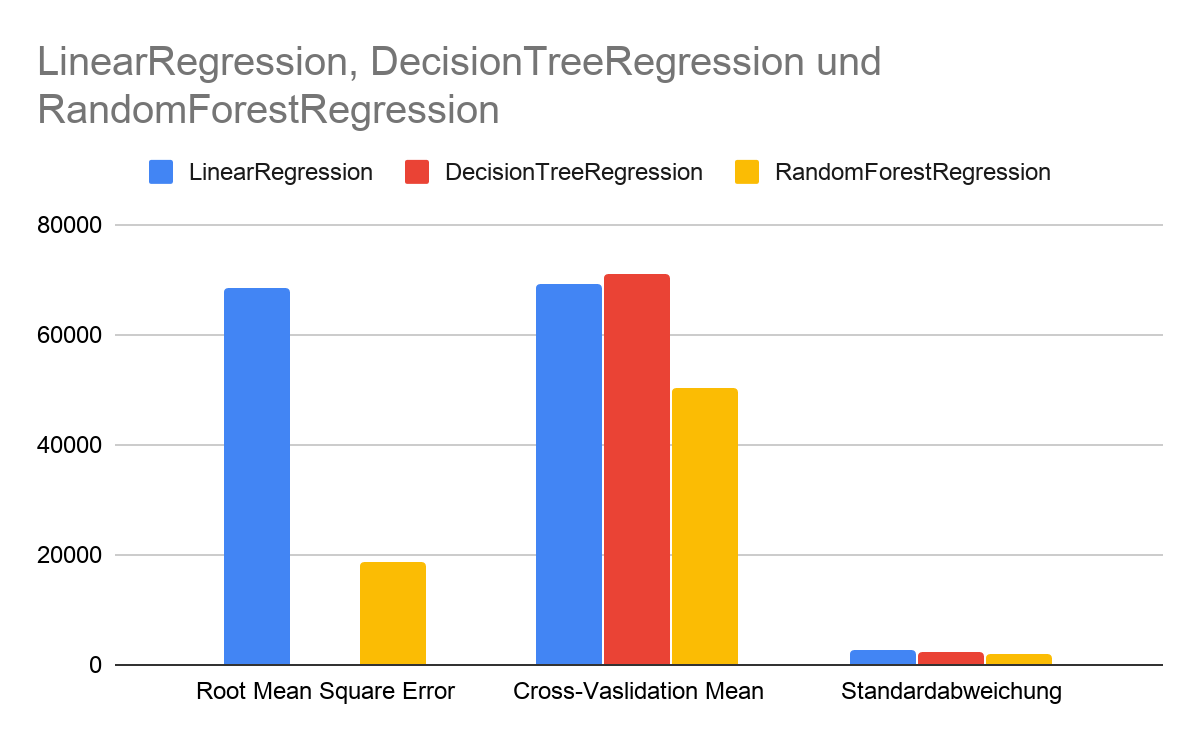
\includegraphics[width=1.0\textwidth]{C:/Users/PitAu/Desktop/Seminar Zeug/MLSKLSeminar/LaTex/Bilder/imageLikeEmbed.png}
	\caption{Statistik: Vergleich verschiedener Algorithmen bei der die y-Achse \$ entspricht}
\end{figure}
Hier lässt sich erkennen, dass für den Algorithmus RandomForestRegression Der Fehler in der Standardabweichung sowie bei der Cross-Validation am kleinsten war, dieser Algorithmus scheint also bisher die genauesten Ergebnisse zu liefern. Dass der Decision-Tree keinen Fehler bei der RMSE-Berechnung hat, liegt also tatsächlich am Overfitting.


\section{Evaluation}
\label{evaluation}
An dieser Stelle wird nun auf das zum Beginn des Projekts erstellte Test-Set zurück gegriffen. Dieses wird genau wie zuvor mit der full\_pipeline vorbereitet, und in Lables und Variablen gesplittet. Mit dem zuvor ausgewählten und trainierten Modell (hier also das RandomForestRegression) wird eine Vorhersage der Median\_House\_Values erstellt und mit den Lables verglichen. Unter Zuhilfenahme der RMSE-Formal aus \hyperlink{datensatz}{Abschnitt 5.3} kann auch hier der RMSE berechnet werden. Das Ergebnis beträgt in dem Experiment 48.464, ein annehmbarer Fehlerwert für die Größenordnung in der wir uns bewegen! Es kann also mithilfe unseren Systems der Preis eines Hauses auf circa \$50.00 richtig geschätzt werden. 
Der Algorithmus RandomForestRegression scheint hierbei die beste Wahl zu sein.


\section{Vergleich mit Classification}
\label{vergleichMitClassification}
Um die verschiedenen Herangehensweisen sinnvoll vergleichen zu können müssen für den Classification-Ansatz zunächst erstmal Klassen definiert werden, in welche die Preise eingeordnet werden sollen. 
Da der Regression-Ansatz ergeben hat, dass Preise durchschnittlich mit einer Genauigkeit von ± \$50.000 bestimmt werden können, sollen hier also Preisklassen von jeweils \$50.000 gebildet werden, somit sollten die Häuser gut in eine richtige Preiskategorie eingestuft werden können. Da nur 156 Preise in die Kategorie <\$50.000 fallen wird diese mit der nächst höheren zu der Kategorie <\$100.000 zusammengefasst.
Als Labels für unsere Daten dienen nun also Integers von 1-10, wobei 10 die höchste Preiskategorie von >\$500000 repräsentiert.
Da nun zwischen 10 verschiedenen Klassen unterschieden werden soll, muss ein mulitclass Classification Algorithmus verwendet werden. Dafür wurde zunächst der Support Vector Machine Algorithmus gewählt. 
Das Verfahren zum Trainieren der Algorithmen ist analog zu dem vorherigen, nur muss hier auf die Auswahl der Labels als Y-Train-Set geachtet werden. 
Beim predicten eines Preises wird dann eine sogenannte decision\_funktion erstellt, mit deren Hilfe sich ein Objekt zu einer Preisklasse zuordnen lassen können soll.
Hier ein Beispiel für solch eine Funktion:
\newline
\begin{figure}
	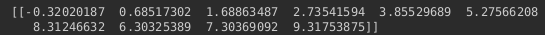
\includegraphics[width=1.0\textwidth]{C:/Users/PitAu/Desktop/Seminar Zeug/MLSKLSeminar/LaTex/Bilder/pasted image 0 (4).png}
	\caption{decision\_funktion}
\end{figure}
In diesem Beispiel ist klar erkennbar, dass der Wert der die Klasse 10 repräsentiert am höchsten ist. Das Objekt sollte aber eigentlich der Klasse 5 zugeordnet werden. 
Hier liegt also ein Fehler vor. Um die Präzision genau zu bestimmen wird wieder mit dem cross\_val\_score gearbeitet.
\newline
\begin{figure}
	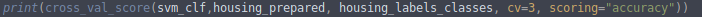
\includegraphics[width=1.0\textwidth]{C:/Users/PitAu/Desktop/Seminar Zeug/MLSKLSeminar/LaTex/Bilder/pasted image 0 (5).png}
	\caption{Code: cross\_val\_score 1}
\end{figure}
\begin{figure}
	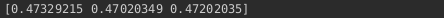
\includegraphics[width=0.7\textwidth]{C:/Users/PitAu/Desktop/Seminar Zeug/MLSKLSeminar/LaTex/Bilder/pasted image 0 (6).png} 
	\caption{Code: cross\_val\_score 2}
\end{figure}
Die Präzision dieses Algorithmus ist mit 47\% nicht besonders gut, weswegen das Problem noch einmal mit einem Classification Algorithmus angegangen wird, der sich bereits bewährt hat: Dem SDGClassifier bzw. dem Random Forest Classifier. Mit diesem Ansatz ließ sich jedoch nur ein Präzision von 35\% erreichen. Um zu zufriedenstellenden Ergebnissen zu gelangen muss also ein anderer Weg gewählt werden. 
\newline
Eine sinnvolle Lösung erschien es uns zu sein, die Preiskategorien anzupassen. Im nächsten Anlauf werden nun Klasses von jeweils \$100.000 benutzt um das System zu trainieren. Es werden also 6 Kategorien erstellt und als Label-Set definiert, mit denen die Algorithmen erneut trainiert und getestet werden. Die Ergebnisse folgen:
\newline
\begin{figure}
	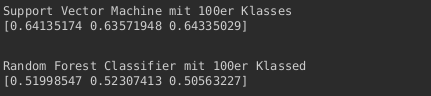
\includegraphics[width=0.7\textwidth]{C:/Users/PitAu/Desktop/Seminar Zeug/MLSKLSeminar/LaTex/Bilder/pasted image 0 (7).png}
	\caption{Ergebnis nach anpassung der Preiskategorien. SVM hat eine Präzision von 64\% und SGD 52\%}
\end{figure}

Bei einer Gegenüberstellung der Ergebnisse des Regressions Ansatzes gegenüber dem Classification Ansatzes lässt sich folgendes festhalten:
\begin{itemize}
\item Mit der Regression ließ sich ein RMSE von \$48.464 erreichen
\item Mit der Classification ließ sich mit 64\% Präzision eine Einordnung in Klassen von jeweils \$100.000 erreichen
\end{itemize}

\section{Projektauswertung}
\label{projektauswertung}
Ein direkter Vergleich dieser Werte ist kaum sinnvoll zu vollziehen.
Der Grund dafür ist uns während der Durchführung des Projekts immer klarer geworden:
Einen direkten Vergleich zwischen Classification- und Regression-Algorithmen ist weder möglich noch sinnvoll. Für jede Problemstellung ist ein anderer Ansatz zu wählen: 
In unserem Beispiel liegt ein klarer Fall von Regression vor, denn es soll ein möglichst genauer Preis für das Haus bestimmt werden. Durch einen Workaround wurde versucht das Problem auch für den Classification Ansatz aufzubereiten, mit diesem erzwungenen Ansatz konnten allerdings keine besonders guten Ergebnisse erzielt werden. Der Clustering-Ansatz ist für den Datensatz so unpassend, dass dieser aus unserem Experiment ausgeschlossen wurde. Ohne das Labeln der Daten werden die Häuser wahrscheinlich in Kategorien wie “Entfernung zum Strand” eingeteilt werden, da diese im Datensatz die klarsten Anzeichen für Klassen zeigen. 
\newline
Jeder Ansatz hat seine Daseinsberechtigung, und dass einige Algorithmen besser abschneiden als andere, kann auch in der Natur der Problemstellung begründet sein. 
Die ersten und wichtigsten Schritte bei einem Machine-Learning Projekt sollten unsere Meinung also folgende sein:
\begin{itemize}
\item Ziel genau definieren \newline
Im Beispiel: Sollen genaue Preise geschätzt werden? Sollen Preisklassen gebildet werden?
\item Visualisierung der Daten \newline
Hier können schon erste wichtige Erkenntnisse gesammelt werden, die ohne die Veranschaulichung vielleicht übersehen werden können.
\item Analyse der Daten \newline
Können schon ohne Machine-Learning Zusammenhänge erkannt werden? 
Wenn ja sollten diese, falls sie für das Projekt sinnvoll erscheinen, unbedingt berücksichtigt werden.
\item Auswahl der Herangehensweise \newline
Mit den Informationen die in den ersten Schritten gesammelt worden, sollte es einfach sein sich für die richtige Methode und den passenden Algorithmus zu entscheiden.
\end{itemize}
Unter Berücksichtigung dieser Gesichtspunkte sollte man meistens zu einer erfolgreichen Algorithmus-Auswahl und damit auch zu einem sinnvollen Projektergebnis gelangen.

\chapter{Resümee}
\label{resümee}
Beim Schreiben dieser Seminararbeit und bei der Durchführung des dazu erdachten Experiments, sahen wir uns immer wieder mit der Vielfältigkeit des Machine-Learnings konfrontiert. 
Unser ursprünglicher Ansatz, der Vergleich verschiedener Algorithmen aus verschiedenen Ansätzen erwies sich mit dem Voranschreiten des Projekts als immer weniger sinnvoll.
Stattdessen haben wir wertvolle Erkenntnisse im Umgang mit Machine Learning Projekten erlangt:
Es gibt keine allgemeingültige beste Lösung, sondern es muss genau überlegt werden welcher Ansatz für das vorliegende Problem der richtige ist. SciKit-Learn unterstützt einen dabei mit zahlreichen Funktionen und Möglichkeiten, die es uns ermöglicht haben die Daten einfach aufzubereiten und zu visualisieren. Diese Tools machen es uns relativ leicht das Problem einzuordnen und dementsprechend die korrekte Herangehensweise zu selektieren.
Bei unserem Projekt ist der sinnvollste Ansatz die Regression, daraus lassen sich allerdings keinerlei Rückschlüsse auf andere Problematiken ziehen.
Mithilfe der gewonnenen Erkenntnisse lässt sich allerdings im Bezug auf das Thema Mobilität eine wichtige Aussage treffen: 
Ein solch umfassendes Thema wie zum Beispiel Autonomes Fahren muss sich aller Instrumente bedienen um ansatzweise abgedeckt werden zu können. Es folgen einige Exempel um diese Aussage zu verdeutlichen.
Als erste Komplexität wollen wir die Erkennung von Straßenschildern nennen. Hier müssen keine unbekannten oder neuen Schilder gedeutet werden, es sind alle Schilder bekannt und können klar gelabelt werden. Hier sollte also unbedingt mit Classification gearbeitet werden um das bestmögliche Ergebnis zu erzielen.
Ein Präzedenzfall für Regression wiederum ist die Berechnung der besten Geschwindigkeit, bei der die Gefährdung minimal ist aber auch der Verkehrsfluss nicht beeinträchtigt wird. Diese ist abhängig vom Abstand zum vorherfahrenden Automobil, der zulässigen Geschwindigkeit, dem Zustand der Fahrbahn und vielen weiteren Faktoren. Aufgrund all dieser Daten muss ein genauer Wert festgelegt werden, es wird also klar, dass Regression hier die sinnvollste Methodik ist. 
All diese Erkenntnisse konnten wir vor allem mithilfe unseres Projekts erlangen. Dieses hat zwar nicht zu den Ergebnissen geführt, die wir uns anfangs erhofft haben, hat dafür aber zu einem tieferen Verständnis für Deep-Learning und dessen Diversität in Ansätzen und Problemen geführt und war deswegen für uns von allergrößter Bedeutung und Nutzen.





































